\documentclass[aspectratio=169]{ISAE-Beamer}
\usefonttheme[onlymath]{serif}
\usepackage{amsmath,amssymb,amsthm}
\usepackage{bm}

\usepackage{graphicx}
\usepackage{diffcoeff}
\usepackage{dsfont}
\usepackage{mathrsfs}
\usepackage{tcolorbox}

%\usepackage{multimedia}
\usepackage{media9}
\usepackage[backend=bibtex]{biblatex}

\graphicspath{{../Figures/}}

\bibliography{bib_pres_IFACWC}

\DeclareMathOperator{\Tr}{Tr}
\DeclareMathOperator*{\grad}{grad}
\DeclareMathOperator*{\Grad}{Grad}
\DeclareMathOperator*{\Div}{Div}
\renewcommand{\div}{\operatorname{div}}
\DeclareMathOperator*{\Hess}{Hess}

\DeclareMathOperator*{\argmax}{arg\,max}
\DeclareMathOperator*{\argmin}{arg\,min}

\def\onedot{$\mathsurround0pt\ldotp$}
\def\cddot{% two dots stacked vertically
	\mathbin{\vcenter{\baselineskip.67ex
			\hbox{\onedot}\hbox{\onedot}}%
}}

\renewcommand\bibfont{\scriptsize}


\makeatletter \renewcommand\d[1]{\ensuremath{%
		\;\mathrm{d}#1\@ifnextchar\d{\!}{}}}
\makeatother

\title[21st IFAC World Congress]{Partitioned finite element method for structured discretization with mixed boundary conditions}

\author[Andrea Brugnoli]{Andrea Brugnoli\inst{1}, Fl\'avio Luiz Cardoso-Ribeiro\inst{2}, Ghislain Haine\inst{1}, Paul Kotyczka\inst{3}}

\institute{\inst{1}ISAE-SUPAERO, France \and \inst{2}Instituto Tecnol\'ogico de Aeron\'autica, Brazil \and \inst{3}Technical University of Munich, Germany}

\date[Berlin, 11/7/20]{July, the 11th, 2020}

%\thanks{}

\begin{document}

\maketitle

\begin{frame}{Outline}

\tableofcontents

\end{frame}

\section{Introduction: problem statement}

\begin{frame}{Model description}
\begin{overlayarea}{\textwidth}{\textheight}
Model for the propagation of sound in air
\begin{equation*}
\diffp{}{t}
\begin{bmatrix}
\chi_s p \\
\mu_0 \bm{v} \\
\end{bmatrix} = -
\begin{bmatrix}
0 & \mathrm{div} \\
\mathrm{grad} & 0 \\
\end{bmatrix}
\begin{bmatrix}
p \\
\bm{v} \\
\end{bmatrix}, \qquad \text{on } \Omega = \{x \in [0, L],\; r \in [0, R],\; \theta = [0, 2 \pi)\}.
\end{equation*}
\only<1>{
\begin{itemize}
\item $p \in \mathbb{R}$  and $\bm{v} \in \mathbb{R}^3$: variations of pressure and velocity from a steady state;
\item $\mu_0$: the steady state mass density;
\item $\chi_s$: adiabatic compressibility factor;
\item $x, r, \theta$: axial, radial and tangential coordinates.
\end{itemize}
}
\only<2>{
\begin{columns}[T]
		\setlength{\abovedisplayskip}{3pt}
		\setlength{\belowdisplayskip}{3pt}
\begin{column}{.45\textwidth}
	Boundary conditions
	\begin{align*}
	p(x, R, \theta) &= - \mathcal{Z}(x, t) \, v_r(x, R, \theta), \\
	\bm{v} \cdot \bm{n}(0, r, \theta) &= -v_x(0, r, \theta) = - f(r), \\
	\bm{v} \cdot \bm{n}(L, r, \theta) &= +v_x(L, r, \theta) = + f(r), 
	\end{align*}
\end{column}
\begin{column}{.45\textwidth}
	Initial conditions
	\begin{equation*}
	\begin{aligned}
	p^0(x, r, \theta) &= 0, \\
	v_x^0(x, r, \theta) &= f(r), 
	\end{aligned}  \qquad
	\begin{aligned}
	v_r^0(x, r, \theta) &= g(r), \\
	v_\theta^0(x, r, \theta) &= 0.
	\end{aligned}    
	\end{equation*}
\end{column}
\end{columns}
\vspace{5pt}
The impedance $\mathcal{Z}$ and the axial $f(r)$ and radial flow $g(r)$ expressions are the following
\begin{equation*}
\begin{aligned}
\mathcal{Z}(x, t) = \mathds{1}\left\{ \frac{1}{3} L \leq \ x \ \leq \frac{2}{3} L, \,  t \geq 0.2 \ t_{\text{fin}} \right\} \mu_0 \, c_0, \\
f(r) = \left( 1 - \frac{r^2}{R^2} \right) v_0, \qquad
g(r) = 16 \frac{r^2}{R^4} \left( R - r \right)^2 v_0. 
\end{aligned}
\end{equation*}
}
\only<3>{
	\centering
	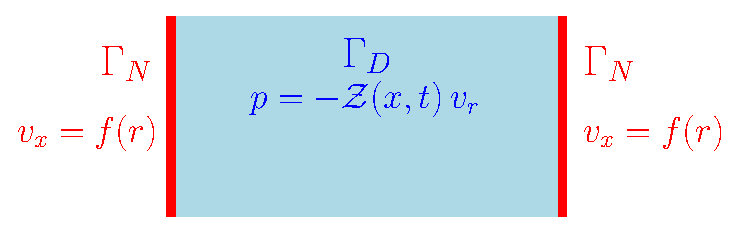
\includegraphics[width=0.8\textwidth]{bc_3D_sketch.eps}	
}
\end{overlayarea}
\end{frame}



\begin{frame}{Model reduction by symmetry}
\begin{overlayarea}{\textwidth}{\textheight}
	
	Because of symmetry the model can be reduced to a 2D problem in polar coordinates over the domain $\Omega_{\text{r}} = \{x \in [0, L], r \in [0, R]\}$
	\begin{equation*}
	\diffp{}{t}
	\begin{bmatrix}
	\chi_s p \\
	\mu_0 v_x \\
	\mu_0 v_r \\
	\end{bmatrix} = -
	\begin{bmatrix}
	0 & \partial_x & \partial_r + 1/r \\
	\partial_x & 0 & 0 \\
	\partial_r & 0 & 0 \\
	\end{bmatrix}
	\begin{bmatrix}
	p \\
	v_x \\
	v_r \\
	\end{bmatrix}.
	\end{equation*}
	\only<2>{
	The boundary conditions must now account for the symmetry condition at $r=0$
				\begin{align*}
				p(x, R, \theta) &= - \mathcal{Z}(x, t) \, v_r(x, R, \theta), \\
				\bm{v} \cdot \bm{n}(0, r, \theta) &= -v_x(0, r, \theta) = - f(r), \\
				\bm{v} \cdot \bm{n}(L, r, \theta) &= +v_x(L, r, \theta) = + f(r), \\
				\bm{v}\cdot \bm{n}(x, 0) &= v_r(x, 0) =0
				\end{align*}	
	}
\only<3>{
	\centering
	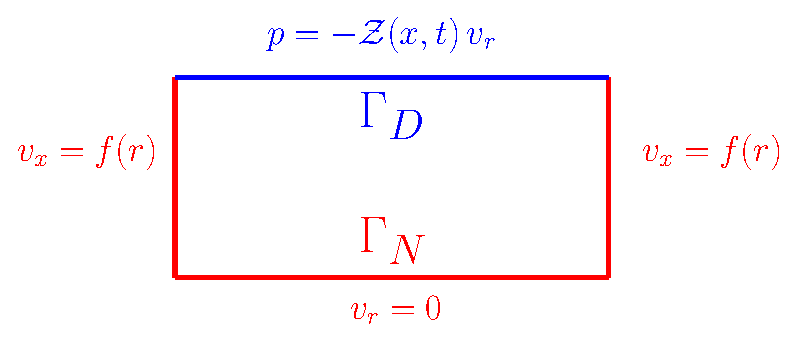
\includegraphics[width=0.7\textwidth]{bc_2D_sketch.eps}	
}
\end{overlayarea}
\end{frame}

\begin{frame}{A port-Hamiltonian structure}
\begin{overlayarea}{\textwidth}{\textheight}
	\setlength{\abovedisplayskip}{8pt}
	\setlength{\belowdisplayskip}{8pt}
The system can be rewritten compactly as a pH system in co-energy variables 
\begin{equation*}
\label{eq:sys_ph}
\mathcal{M} \partial_t{e} = \mathcal{J} e
\end{equation*}
where $\mathcal{M} = \mathrm{diag}([\chi_s, \ \mu_0, \ \mu_0])$  and $e = [p, \ v_x, \ v_r]^\top$. \\
\vspace{8pt}
\only<1>{
The Hamiltonian is then computed as
\[
H = \frac{1}{2} \left(e, \mathcal{M} e  \right)_{\Omega_{\text{r}}}
\]
where $\left(\cdot, \cdot \right)_{\Omega_{\text{r}}}$ is the standard $L^2$ inner product in polar coordinates
\[
\left(\alpha, \beta \right)_{\Omega_{\text{r}}} = \int_{\Omega_{\text{r}}} \alpha \cdot \beta \ r \d{r} \d{x} = \int_{\Omega_{\text{r}}} \alpha \cdot \beta \ \d{\Omega_r}.
\]
The power flow is obtained by application of the Stokes theorem
\[
\dot{H} =  - \int_{0}^{L} \mathcal{Z}(x, t) v_r^2 \ R \d{x} \le 0 
\]
}
\only<2>{
The interconnection operator $\mathcal{J}$ can be decomposed into the sum of $\mathcal{J} = \mathcal{J}_{\text{div}} + \mathcal{J}_{\text{grad}}$
\begin{equation*}
\mathcal{J}_{\text{div}} = -\begin{bmatrix}
0 & \partial_x & \partial_r + 1/r \\
0 & 0 & 0 \\
0 & 0 & 0 \\
\end{bmatrix}, \qquad 
\mathcal{J}_{\text{grad}} = -\begin{bmatrix}
0 & 0 & 0 \\
\partial_x & 0 & 0 \\
\partial_r & 0 & 0 \\
\end{bmatrix}.
\end{equation*}
}
\end{overlayarea}
\end{frame}


\section{Finite element Discretization}

\begin{frame}{}
\begin{exampleblock}{Available methods}
	\begin{itemize}
		\item Spectral methods (Moulla 2012):
		\begin{itemize}
			\item[\textcolor{green}{\checkmark}] Rapid spectral convergence;
			\item[\textcolor{red}{$\times$}] Only for 1D problem;
		\end{itemize}
		\item Finite differences (Trenchant 2018);
		\begin{itemize}
			\item[\textcolor{green}{\checkmark}] Valid up to 2D geometries;
			\item[\textcolor{red}{$\times$}] Requires \textit{ad hoc} implementation (staggered grids);
		\end{itemize}
		\item Finite elements based
		\begin{itemize}
			\item Golo 2004, Kotyczka 2018: the implementation requires exterior calculus knowledge and depends on the some parameters that ensure the preservation of power flow;		
			\item \textcolor{blue}{Cardoso-Ribeiro 2018}:
			\begin{itemize}
				\item[\textcolor{green}{\checkmark}] Natural extension of the mixed finite element method to pH systems;
				\item[\textcolor{green}{\checkmark}] Implementable using well-established libraries (Fenics, Firedrake);
			\end{itemize}
		\end{itemize}
	\end{itemize}
\end{exampleblock}
\end{frame}

\begin{frame}{The partitioned finite element method (PFEM)}

\begin{block}{General procedure for PFEM}
	\setlength{\abovedisplayskip}{1pt}
	\setlength{\belowdisplayskip}{1pt}
	\begin{enumerate}
		\item Put the system into weak form:
		\begin{equation*}
		\left(v, \mathcal{M} \diffp{e}{t} \right)_{\Omega} = \left(v, \mathcal{J} e \right)_{\Omega}.
		\end{equation*}
		\item Apply integration by part on a partition of $\mathcal{J}$:
		\begin{equation*}
		\left(v, \mathcal{J} e \right)_{\Omega} \overbrace{=}^{i.b.p.} j(v, e)_{\Omega} + b(v, u_\partial)_{\partial \Omega},
		\end{equation*}
		so that $j(v, e)_{\Omega}$ is a skew-symmetric bilinear form.
		\item Discretization by Galerkin method (same basis function for test and co-energy variables)
	\end{enumerate}
\end{block}
\end{frame}

\begin{frame}{Application to the wave equation}
\only<1>{
If the integration by parts is applied on $\mathcal{J}_{\text{div}}$
\begin{equation*}
\left(w, \mathcal{J} e \right)_{\Omega_{\text{r}}} = \left(w, \mathcal{J}_{\text{grad}} \ e \right)_{\Omega_{\text{r}}} - \left(\mathcal{J}_{\text{grad}} \ w, e \right)_{\Omega_{\text{r}}} + \left(w_p, \textcolor{red}{u_N} \right)_{\partial \Omega_{\text{r}}}.
\end{equation*}
The skew-symmetric bilinear form 
\[ j_{\text{grad}}(w, e) := \left(w, \mathcal{J}_{\text{grad}} \ e \right)_{\Omega_{\text{r}}} - \left(\mathcal{J}_{\text{grad}} \ w, e \right)_{\Omega_{\text{r}}} \]
may now be introduced, together with the boundary form
\begin{equation*}
\label{eq:f_N}
\left(w_p, u_N \right)_{\partial \Omega_{\text{r}}} = \int_{\partial \Omega_{\text{r}}} w_p \textcolor{red}{u_N} \ \d{\Gamma_r},
\end{equation*}
where $\textcolor{red}{u_N} = \bm{v} \cdot \bm{n} \vert_{\partial \Omega_r}$. The corresponding power conjugated output is given by $\textcolor{blue}{y_N} = p \vert_{\partial \Omega_r}$. \\
The system in weak form under Neumann boundary control is then written as
\begin{equation*}
\label{eq:wf_grad}
\begin{aligned}{}
(w, \mathcal{M} \partial_t{e})_{\Omega_{\text{r}}} &= j_{\text{grad}}(w, e) + \left(w_p, \textcolor{red}{u_N} \right)_{\partial \Omega_{\text{r}}}. \\
\left(w_N, \textcolor{blue}{y_N} \right)_{\partial \Omega_{\text{r}}} &= \left(w_N, p \right)_{\partial \Omega_{\text{r}}},
\end{aligned}
\end{equation*}
}


\only<2>{
If the integration by parts is carried out on $\mathcal{J}_{\text{grad}}$ 
\begin{equation*}
\left(w, \mathcal{J} e \right)_{\Omega_{\text{r}}} = \left(v, \mathcal{J}_{\text{div}} \ e \right)_{\Omega_{\text{r}}} - \left(\mathcal{J}_{\text{div}} \ w, e \right)_{\Omega_{\text{r}}} + \left(\bm{w}_v \cdot \bm{n}, \textcolor{blue}{u_D} \right)_{\partial \Omega_{\text{r}}}.
\end{equation*}
The skew-symmetric bilinear form 
\[ j_{\text{div}}(w, e) := \left(w, \mathcal{J}_{\text{div}} \ e \right)_{\Omega_{\text{r}}} - \left(\mathcal{J}_{\text{div}} \ w, e \right)_{\Omega_{\text{r}}} \]
is introduced, together with the boundary form
\begin{equation*}
\left(\bm{w}_v \cdot \bm{n}, \textcolor{blue}{u_D} \right)_{\partial \Omega_{\text{r}}} = \int_{\partial \Omega_{\text{r}}} \bm{w}_v \cdot \bm{n} \ \textcolor{blue}{u_D} \ \d{\Gamma_r}, 
\end{equation*}
where $\textcolor{blue}{u_D} = p \ \vert_{\partial \Omega_r}$. Adding  the conjugated output $\textcolor{red}{y_D} = \bm{v}\cdot~\bm{n}\vert_{\partial \Omega_r}$, the system in weak form under Dirichlet boundary control is then written as
\begin{equation*}
\label{eq:wf_div}
\begin{aligned}
(w, \mathcal{M} \partial_t{e})_{\Omega_{\text{r}}} &= j_{\text{div}}(w, e) + \left(\bm{w}_v \cdot \bm{n}, \textcolor{blue}{u_D} \right)_{\partial \Omega_{\text{r}}}, \\
\left(w_D, \textcolor{red}{y_D} \right)_{\partial \Omega_{\text{r}}} &= \left(w_D, \bm{v}\cdot\bm{n} \right)_{\partial \Omega_{\text{r}}},
\end{aligned}
\end{equation*}
}
\end{frame}

\begin{frame}{Mixed boundary condition}

To tackle mixed boundary conditions two approaches are developed
\begin{itemize}
	\item A Lagrange multiplier based method;
	\item A virtual domain decomposition method.
\end{itemize} 	
\end{frame}

\subsection{Lagrange multiplier approach}

\begin{frame}
Start from 
\begin{equation*}
\left(w, \mathcal{J} e \right)_{\Omega_{\text{r}}} = \left(w, \mathcal{J}_{\text{grad}} \ e \right)_{\Omega_{\text{r}}} - \left(\mathcal{J}_{\text{grad}} \ w, e \right)_{\Omega_{\text{r}}} + \left(w_p, \bm{v}\cdot\bm{n}\vert_{\partial \Omega_{\text{r}}} \right)_{\partial \Omega_{\text{r}}}.
\end{equation*}
	The quantity $\bm{v}\cdot\bm{n}\vert_{\partial \Omega_{\text{r}}}$ is known only $\Gamma_N$. On $\Gamma_D$ a Lagrange multiplier $\lambda_D$ is introduced 
	\begin{equation}
	\label{eq:bdint_dae}
	\int_{\partial \Omega_{\text{r}}} w_p \bm{v} \cdot \bm{n} \d{\Gamma_r} = \int_{\Gamma_N} w_p u_N \ \d{\Gamma_r} + \int_{\Gamma_D} w_p \lambda_D \d{\Gamma_r}.
	\end{equation}
	The constraint associated with the Lagrange multiplier  is the non-homogeneous Dirichlet condition
	\begin{equation}
	\label{eq:wf_con}
	\int_{\Gamma_D} w_\lambda (p - u_D) \d{\Gamma_r} = 0, \qquad \text{$w_\lambda$ test function for the Lagrange multiplier.}
	\end{equation}
	
	\begin{block}{Final Weak Form}
	\begin{equation*}
\begin{aligned}
m(w, \partial_t{e}) &= j_{\text{grad}}(w, e) + \left(w_p, \lambda_D \right)_{\Gamma_D} + \left(w_p, u_N \right)_{\Gamma_N}, \\
0 &= - \left(w_\lambda, p \right)_{\Gamma_D} + \left(w_\lambda, u_D \right)_{\Gamma_D}, \\
\left(w_N, y_N \right)_{\Gamma_N} &= \left(w_N, p \right)_{\Gamma_N}, \\
\left(w_D, y_D \right)_{\Gamma_D} &= \left(w_D, \lambda_D \right)_{\Gamma_D}, 
\end{aligned}
\end{equation*}
	\end{block}


\end{frame}

\begin{frame}
		where $w_N, w_D$ are the test functions associated to the output discretization and $\left( \cdot, \cdot \right)_{\Gamma_{*}}$ is the $L^2$ inner product on boundary $\Gamma_*$. A Galerkin method can now be applied to retrieve a finite dimensional pH system. This means that corresponding test and trial functions are discretized using the same basis
	\begin{equation}
	\label{eq:basis_func}
	\begin{aligned}
	\begin{aligned}
	p &\approx \sum_{i=1}^{n_p} \phi_p^i(x, r) p^i, \\
	\bm{v} &\approx \sum_{i=1}^{n_v} \bm\phi_v^i(x, r) v^i, \\
	\end{aligned} \quad
	\begin{aligned}
	*_D &\approx \sum_{i=1}^{n_D} \phi^i_\Gamma(s) *^i_D, \quad (* = \{u, y, \lambda\}), \\
	*_N &\approx \sum_{i=1}^{n_N} \phi_\Gamma^i(s) *^i_N, \quad (* = \{u,  y\}).
	\end{aligned} 
	\end{aligned}
	\end{equation}
	The shape functions $\phi_p^i(x, r), \bm\phi_v^i(x, r)$ are defined over the domain, whereas $\phi_\Gamma^i(s)$ ($s$ is the curvilinear abscissa) is defined on the boundary only. Plugging the approximations \eqref{eq:basis_func} into \eqref{eq:weak_lag}, a pHDAE (\cite{beattie2018linear}) is obtained:
	\begin{equation}
	\begin{aligned}
	\label{eq:discr_phdae}
	\begin{bmatrix}
	\mathbf{M} & \mathbf{0} \\
	\mathbf{0} & \mathbf{0} \\
	\end{bmatrix} \frac{\d}{\d t}
	\begin{bmatrix}
	\mathbf{e}\\
	\bm{\lambda}_D \\
	\end{bmatrix}
	&= \begin{bmatrix}
	\mathbf{J} & \mathbf{G}_D\\
	-\mathbf{G}_D^T & \mathbf{0} \\
	\end{bmatrix}
	\begin{bmatrix}
	\mathbf{e}\\
	\bm{\lambda}_D \\
	\end{bmatrix} + \begin{bmatrix}
	\mathbf{B}_N & \mathbf{0}\\
	\mathbf{0} & \mathbf{B}_D \\
	\end{bmatrix}
	\begin{bmatrix}
	\mathbf{u}_N \\
	\mathbf{u}_D \\
	\end{bmatrix}, \\
	\begin{bmatrix}
	\mathbf{y}_N \\
	\mathbf{y}_D \\
	\end{bmatrix} &=
	\begin{bmatrix}
	\mathbf{B}_N^T & \mathbf{0} \\ 
	\mathbf{0} & \mathbf{B}_D^T \\ 
	\end{bmatrix}
	\begin{bmatrix}
	\mathbf{e}\\
	\bm{\lambda}_D \\
	\end{bmatrix},
	\end{aligned}
	\end{equation}
	where $\mathbf{M} = \mathrm{diag}(\mathbf{M}_p, \mathbf{M}_v)$ and
	\begin{equation*}
	\mathbf{J} = \begin{bmatrix}
	\mathbf{0} & \mathbf{A}_{\mathrm{grad}} \\
	- \mathbf{A}_{\mathrm{grad}}^T & \mathbf{0} \\
	\end{bmatrix}, \quad 
	\mathbf{G}_{D} = \begin{bmatrix}
	\mathbf{G}_{D, p} \\
	\mathbf{0} \\
	\end{bmatrix}, \quad
	\mathbf{B}_{N} = \begin{bmatrix}
	\mathbf{B}_{N, p} \\
	\mathbf{0} \\
	\end{bmatrix}.
	\end{equation*}
	The matrices elements are computed as follows:
	\begin{equation*}
	\begin{aligned}
	\mathbf{M}_p^{ij} &= ({\phi}_{p}^i,\, \chi_s {\phi}_{p}^j)_{\Omega_r}, \\ \mathbf{M}_v^{ij} &= (\bm{\phi}_{v}^i,\, \mu_0 \bm{\phi}_{v}^j)_{\Omega_r}, \\
	\mathbf{A}_{\mathrm{grad}}^{ij} &= (\nabla{\phi}_{p}^{i}, \, \bm{\phi}_{v}^j)_{\Omega_r}, 
	\end{aligned} \quad 
	\begin{aligned}
	\mathbf{G}_{D, p}^{ij} &= ({\phi}_{p}^i,\, {\phi}_{\Gamma}^j)_{\Gamma_D}, \\ 
	\mathbf{B}_{N, p}^{ij} &= ({\phi}_{p}^{i},\, {\phi}_{\Gamma}^{j})_{\Gamma_N}, \\
	\mathbf{B}_{D}^{ij} &= ({\phi}_{\Gamma}^{i},\, {\phi}_{\Gamma}^{j})_{\Gamma_D}. \\
	\end{aligned}
	\end{equation*}
	
	
	Concerning the actual boundary conditions, on $\Gamma_D$ the impedance condition \eqref{eq:bc_imp} is applied while on  $\Gamma_N$ the inlet and outlet flow condition \eqref{eq:bc_flowL}, \eqref{eq:bc_flowR} hold on the left and right side of the rectangle. The impedance boundary conditions is imposed by putting into weak form the expression $u_D=-\mathcal{Z}\lambda_D=-\mathcal{Z}y_D$:
	\[ \mathbf{M}_{\Gamma_D} \mathbf{u}_D = - \mathbf{M}_{\Gamma_D, \mathcal{Z}} \widehat{\mathbf{y}}_D,
	\]
	where $\mathbf{M}_{\Gamma_D, \mathcal{Z}}$ corresponds to the mass matrix associated to the weighted inner product $\left(w_D, \mathcal{Z}  y_D\right)_{\Gamma_D}$, namely $\mathbf{M}_{\Gamma_D, \mathcal{Z}}^{ij} = \left(\phi_\Gamma^i, \mathcal{Z}  \phi_\Gamma^j \right)_{\Gamma_D}$. This amounts to applying to system \eqref{eq:sys_dae} the control law
	\[ \mathbf{u}_D = - \mathbf{M}_{\Gamma_D}^{-1} \mathbf{M}_{\Gamma_D, \mathcal{Z}} \mathbf{M}_{\Gamma_D}^{-1} \mathbf{y}_D = -\mathbf{Z} \mathbf{y}_D.
	\]
	The Neumann boundary condition is imposed by projection on the $u_N$ space.   The boundary controlled system becomes   
	\begin{equation}
	\label{eq:sys_dae}
	\begin{bmatrix}
	\mathbf{M} & \mathbf{0} \\
	\mathbf{0} & \mathbf{0} \\
	\end{bmatrix} \frac{\d}{\d t}
	\begin{bmatrix}
	\mathbf{e}\\
	\bm{\lambda}_D \\
	\end{bmatrix}
	= \begin{bmatrix}
	\mathbf{J} & \mathbf{G}_D\\
	-\mathbf{G}_D^T & -\mathbf{R} \\
	\end{bmatrix}
	\begin{bmatrix}
	\mathbf{e}\\
	\bm{\lambda}_D \\
	\end{bmatrix} + \begin{bmatrix}
	\mathbf{b}_N \\
	\mathbf{0} \\
	\end{bmatrix},
	\end{equation}
	with $\mathbf{R} = \mathbf{B}_D \mathbf{Z} \mathbf{B}_D^T$ a symmetric positive definite matrix. 
	
\end{frame}


\subsection{Virtual domain decomposition}



\begin{frame}{Results}
\begin{center}
	\onslide*<1>{
		\begin{columns}
			\begin{column}{.3\textwidth}
				\includemedia[
				label=vidNoRod,
				addresource=../Videos/wave_dae15.mp4,
				activate=pageopen,
				width=4cm, height=5cm,
				flashvars={
					source=../Videos/wave_dae15.mp4
					&loop=true
				}
				]{}{VPlayer.swf}
				DAE $h = L/15$
			\end{column}		
			\begin{column}{.3\textwidth}
				\includemedia[
				label=vidNoRod,
				addresource=../Videos/wave_dae10.mp4,
				activate=pageopen,
				width=4cm, height=5cm,
				flashvars={
					source=../Videos/wave_dae10.mp4
					&loop=true
				}
				]{}{VPlayer.swf}
				DAE $h = L/10$
			\end{column}
			\begin{column}{.3\textwidth}
				\includemedia[
				label=vidRod,
				addresource=../Videos/wave_ode10.mp4,
				activate=pageopen,
				width=4cm, height=5cm,
				flashvars={
					source=../Videos/wave_ode10.mp4
					&loop=true
				}
				]{}{VPlayer.swf}
				ODE $h = L/10$
			\end{column}
		\end{columns}
	
	\mediabutton[
	mediacommand=vidNoRod:playPause,
	mediacommand=vidRod:playPause
	]{\fbox{Play/Pause}}
				
		%\movie[width=0.8\textwidth, height=0.6\textheight]{Plate and rod}{../Videos/Comparison_RodNoRod.mp4}	
	}
		\onslide*<2>{
		
		}
	\end{center}
\end{frame}


\end{document}
